\documentclass[tikz,border=7pt]{standalone}
\usepackage{amsmath,amssymb}
\usetikzlibrary{arrows.meta,calc,positioning,decorations.pathreplacing}

% ============================================================
% FOUR explicit, sphere-specialized figures at p = (0,0,1):
%   (1) Gauss map  N:S^2->S^2,  p |-> p (outward normal)
%   (2) Differential (dN)_p computed from a concrete curve gamma(t)
%   (3) Identification of planes:  T_pS^2 = (N(p))^\perp = T_{N(p)}S^2  inside R^3
%   (4) Shape operator S_p = -(dN)_p and its diagonal matrix in a chosen basis
%
% For clarity, (1),(2),(4) use the xz cross-section (y=0) where S^2 is the unit circle.
% Figure (3) uses a clean 3D-style schematic: the plane z=1 through p.
% ============================================================

\begin{document}
	
	% ============================================================
	% (1) Gauss map N: S^2 -> S^2, N(p)=p  (identity map)
	% ============================================================
	\begin{tikzpicture}[>=Latex, line cap=round, line join=round, scale=3.8]
		
		\begin{scope}[shift={(0,0)}]
			\draw[thick] (0,0) circle (1);
			\node at (0,1.28) {$S^2$ (domain)};
			\draw[->] (-1.15,0) -- (1.15,0) node[below] {$x$};
			\draw[->] (0,-0.15) -- (0,1.35) node[left] {$z$};
			
			\coordinate (pL) at (0,1);
			\fill (pL) circle (0.9pt) node[above left] {$p=(0,0,1)$};
			
			% outward normal N(p)=p (radial)
			\draw[very thick,->] (pL) -- ++(0,0.35) node[above] {$N(p)=p$};
			
			\node[align=left] at (-1.13,0.75) {$N:S^2\to S^2$\\[-2pt] $p\mapsto p$};
		\end{scope}
		
		\begin{scope}[shift={(3.1,0)}]
			\draw[thick] (0,0) circle (1);
			\node at (0,1.28) {$S^2$ (codomain)};
			\draw[->] (-1.15,0) -- (1.15,0) node[below] {$x$};
			\draw[->] (0,-0.15) -- (0,1.35) node[left] {$z$};
			
			\coordinate (pR) at (0,1);
			\fill (pR) circle (0.9pt) node[above right] {$N(p)=p$};
			\draw[->] (0,0) -- (pR);
		\end{scope}
		
		\draw[very thick,->] (1.15,1.02) -- (1.95,1.02) node[midway, above] {$N$};
		
	\end{tikzpicture}
	
	\vspace{10pt}
	
	% ============================================================
	% (2) Differential (dN)_p : computed via a concrete curve gamma(t)
	% ============================================================
	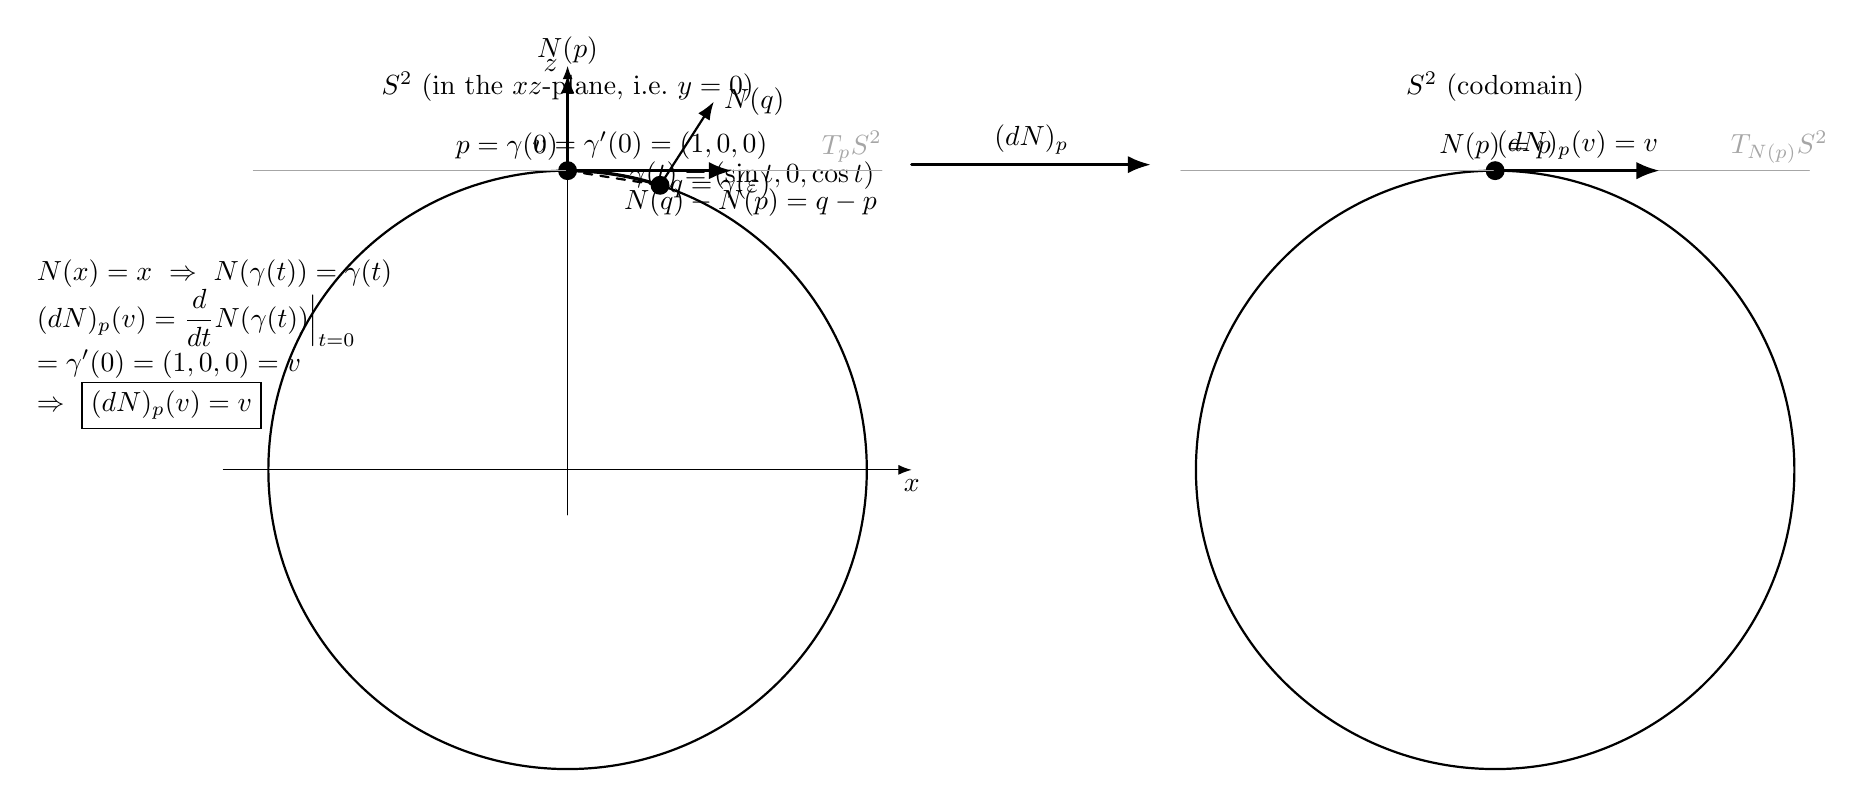
\begin{tikzpicture}[>=Latex, line cap=round, line join=round, scale=3.8]
		
		\def\epsdeg{18}
		\pgfmathsetmacro{\sE}{sin(\epsdeg)}
		\pgfmathsetmacro{\cE}{cos(\epsdeg)}
		\pgfmathsetmacro{\epsrad}{\epsdeg*pi/180}
		
		\begin{scope}[shift={(0,0)}]
			\draw[thick] (0,0) circle (1);
			\node at (0,1.28) {$S^2$ (in the $xz$-plane, i.e.\ $y=0$)};
			\draw[->] (-1.15,0) -- (1.15,0) node[below] {$x$};
			\draw[->] (0,-0.15) -- (0,1.35) node[left] {$z$};
			
			\coordinate (p) at (0,1);
			\coordinate (q) at (\sE,\cE);
			
			\fill (p) circle (0.9pt) node[above left] {$p=\gamma(0)$};
			\fill (q) circle (0.9pt) node[right] {$q=\gamma(\varepsilon)$};
			
			% gamma(t) = (sin t, 0, cos t)
			\draw[very thick]
			(p) arc[start angle=90, end angle=90-\epsdeg, radius=1]
			node[pos=0.55, right] {$\gamma(t)=(\sin t,0,\cos t)$};
			
			% tangent line at p (horizontal)
			\draw[gray!70] (-1.05,1) -- (1.05,1);
			\node[gray!70] at (0.95,1.08) {$T_pS^2$};
			
			% tangent vector v = gamma'(0) = (1,0,0)
			\draw[very thick,->] (p) -- ++(0.55,0) node[midway, above] {$v=\gamma'(0)=(1,0,0)$};
			
			% normals: N(p)=p, N(q)=q (since N=Id)
			\draw[thick,->] (p) -- ++(0,0.32) node[above] {$N(p)$};
			\draw[thick,->] (q) -- ++(0.18,0.28) node[right] {$N(q)$};
			
			% chord q-p = N(q)-N(p)
			\draw[thick,dashed] (p) -- (q) node[midway, below right] {$N(q)-N(p)=q-p$};
			
			% computation annotation
			\node[align=left] at (-1.18,0.42) {%
				$\displaystyle N(x)=x\ \Rightarrow\ N(\gamma(t))=\gamma(t)$\\
				$\displaystyle (dN)_p(v)=\frac{d}{dt}N(\gamma(t))\Big|_{t=0}$\\
				$\displaystyle =\gamma'(0)= (1,0,0)=v$\\
				$\displaystyle\Rightarrow\ \boxed{(dN)_p(v)=v}$};
		\end{scope}
		
		% Right: tangent space at N(p)=p (same horizontal line)
		\begin{scope}[shift={(3.1,0)}]
			\draw[thick] (0,0) circle (1);
			\node at (0,1.28) {$S^2$ (codomain)};
			\coordinate (np) at (0,1);
			\fill (np) circle (0.9pt) node[above] {$N(p)=p$};
			
			\draw[gray!70] (-1.05,1) -- (1.05,1);
			\node[gray!70] at (0.95,1.08) {$T_{N(p)}S^2$};
			
			\draw[very thick,->] (np) -- ++(0.55,0) node[midway, above] {$(dN)_p(v)=v$};
		\end{scope}
		
		\draw[very thick,->] (1.15,1.02) -- (1.95,1.02) node[midway, above] {$(dN)_p$};
		
	\end{tikzpicture}
	
	\vspace{10pt}
	
	% ============================================================
	% (3) Identification:  T_pS^2 = (N(p))^\perp = T_{N(p)}S^2  inside R^3
	% Shown as the plane z=1 at p=(0,0,1) and the orthogonality to N(p).
	% ============================================================
	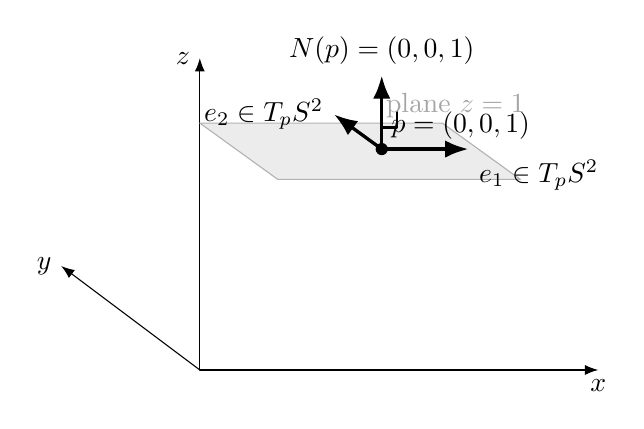
\begin{tikzpicture}[>=Latex, line cap=round, line join=round, scale=1.1]
		
		% 3D-ish schematic in 2D: draw axes and the plane z=1 as a parallelogram
		\coordinate (O) at (0,0);
		\draw[->] (O) -- (4.6,0) node[below] {$x$};
		\draw[->] (O) -- (0,3.6) node[left] {$z$};
		\draw[->] (O) -- (-1.6,1.2) node[left] {$y$};
		
		% plane z=1 represented by a tilted parallelogram
		\coordinate (A) at (0.9,2.2);
		\coordinate (B) at (3.7,2.2);
		\coordinate (C) at (2.8,2.85);
		\coordinate (D) at (0.0,2.85);
		
		\fill[gray!15] (A)--(B)--(C)--(D)--cycle;
		\draw[gray!60] (A)--(B)--(C)--(D)--cycle;
		
		% point p on the plane (center-ish)
		\coordinate (p3) at (2.1,2.55);
		\fill (p3) circle (2pt) node[above right] {$p=(0,0,1)$};
		
		% normal N(p) vertical
		\draw[very thick,->] (p3) -- ++(0,0.85) node[above] {$N(p)=(0,0,1)$};
		
		% two basis vectors in the plane (tangent directions)
		\draw[very thick,->] (p3) -- ++(1.0,0) node[below right] {$e_1\in T_pS^2$};
		\draw[very thick,->] (p3) -- ++(-0.55,0.40) node[left] {$e_2\in T_pS^2$};
		
		% orthogonality marker (schematic)
		\draw[thick] ($(p3)+(0,0.25)$) -- ++(0.18,0) -- ++(0,0.18);
		
%		% labels: identification of tangent spaces
%		\node[align=left] at (4.9,2.55) {%
%			Inside $\mathbb R^3$:
%			\[
%			T_pS^2=\{w:w\cdot N(p)=0\}
%			\]
%			Also
%			\[
%			T_{N(p)}S^2=\{w:w\cdot N(p)=0\}.
%			\]
%			So \(\boxed{T_pS^2=T_{N(p)}S^2=(N(p))^\perp}\).
%		};
		
		\node[gray!70] at (2.95,3.05) {plane $z=1$};
		
	\end{tikzpicture}
	
	\vspace{10pt}
	
	% ============================================================
	% (4) Shape operator: S_p = -(dN)_p, S_p(v)=-v, diagonal matrix -I
	% ============================================================
	\begin{tikzpicture}[>=Latex, line cap=round, line join=round, scale=3.8]
		
		% Left: at p on the circle
		\begin{scope}[shift={(0,0)}]
			\draw[thick] (0,0) circle (1);
			\node at (0,1.28) {$S^2$};
			
			\draw[->] (-1.15,0) -- (1.15,0) node[below] {$x$};
			\draw[->] (0,-0.15) -- (0,1.35) node[left] {$z$};
			
			\coordinate (p) at (0,1);
			\fill (p) circle (0.9pt) node[above left] {$p$};
			
			\draw[gray!70] (-1.05,1) -- (1.05,1);
			\node[gray!70] at (0.95,1.08) {$T_pS^2$};
			
			\draw[thick,->] (p) -- ++(0,0.32) node[above] {$N(p)$};
			
			\draw[very thick,->] (p) -- ++(0.55,0) node[midway, above] {$v$};
			\draw[very thick,->] (p) -- ++(-0.55,0) node[midway, above] {$S_p(v)=-v$};
			
			\node[align=left] at (-1.15,0.43) {%
				$\displaystyle S_p:T_pS^2\to T_pS^2$\\
				$\displaystyle S_p(v)=-(dN)_p(v)$\\
				$\displaystyle (dN)_p(v)=v$};
		\end{scope}
		
		% Right: linear algebra view in basis {e1,e2}
		\begin{scope}[shift={(3.1,0)}]
			\node at (0,1.28) {Choose basis \(\{e_1,e_2\}\) of \(T_pS^2\)};
			
			\coordinate (O2) at (0,0.25);
			\draw[->] (O2) -- ++(1.0,0) node[below right] {$e_1$};
			\draw[->] (O2) -- ++(0,1.0) node[above left] {$e_2$};
			
			\draw[very thick,->] (O2) -- ++(-0.75,0) node[below left] {$S_p(e_1)=-e_1$};
			\draw[very thick,->] (O2) -- ++(0,-0.75) node[below] {$S_p(e_2)=-e_2$};
			
			\node[align=center] at (0,0.95) {$\displaystyle [S_p]_{\{e_1,e_2\}}
				=\begin{pmatrix}-1&0\\[2pt]0&-1\end{pmatrix}$};
			
			\node[align=center] at (0,-0.05) {\(\displaystyle\boxed{S_p=-\mathrm{Id}}\)};
		\end{scope}
		
		\draw[very thick,->] (1.15,1.02) -- (1.95,1.02)
		node[midway, above] {diagonalize};
		
	\end{tikzpicture}
	
\end{document}
